\subsection{\eth}
\label{sec:eth}

\subsubsection{Wprowadzenie}

W pierwszej części ćwiczenia skonfigurowano standardowe połączenie \eth. Jeden z
interfejsów był już skonfigurowany i udostępniał sprawne połączenie do
stacjonarnej sieci w laboratorium, ponieważ przez niego zabootowano system na
maszynie.

Sprawdzono, jakie interfejsy są dostępne.

\begin{lstlisting}
k9% ifconfig -a
sk0: flags=8843<UP,BROADCAST,RUNNING,SIMPLEX,MULTICAST> metric 0 mtu 1500
    options=80009<RXCSUM,VLAN_MTU,LINKSTATE>
    ether 00:11:d8:44:a4:37
    inet 194.29.146.189 netmask 255.255.255.0 broadcast 194.29.146.255
    media: Ethernet autoselect (100baseTX <full-duplex>)
    status: active
ipfw0: flags=8801<UP,SIMPLEX,MULTICAST> metric 0 mtu 65536
lo0: flags=8049<UP,LOOPBACK,RUNNING,MULTICAST> metric 0 mtu 16384
    options=3<RXCSUM,TXCSUM>
    inet 127.0.0.1 netmask 255.0.0.0
\end{lstlisting}

Do pracy z siecią skonfigurowany jest tylko interfejs \texttt{sk0}. Posiada już
pełną konfigurację na 3. wartwie OSI. Przynależy do sieci
\texttt{194.29.146.0/24}. Do tej sieci należy też maszyna \volt{} wykorzystując
swój interfejs \texttt{bge1}. Schemat opisanej konfiguracji znajduje się na
stronie \pageref{fig:eth:schemat-bez-konfiguracji}.

\begin{lstlisting}
volt% ifconfig -a
[...]
bge1: flags=8943<UP,BROADCAST,RUNNING,PROMISC,SIMPLEX,MULTICAST> metric 0 mtu 1500
    options=8009b<RXCSUM,TXCSUM,VLAN_MTU,VLAN_HWTAGGING,VLAN_HWCSUM,LINKSTATE>
    ether 00:e0:81:65:37:d4
    inet 194.29.146.3 netmask 255.255.255.0 broadcast 194.29.146.255
    inet 194.29.146.4 netmask 255.255.255.255 broadcast 194.29.146.4
    inet 194.29.146.11 netmask 255.255.255.255 broadcast 194.29.146.11
    media: Ethernet autoselect (1000baseT <full-duplex>)
    status: active
\end{lstlisting}

\begin{figure}[h!]
  \centering
  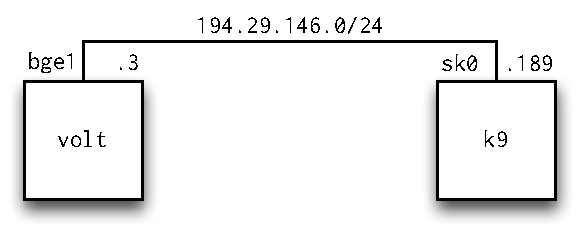
\includegraphics{figury/ethernet/schemat-bez-konfiguracji.pdf}
  \caption{Schemat początkowego połączenia \eth.}
  \label{fig:eth:schemat-bez-konfiguracji}
\end{figure}

Z wydruku \texttt{ifconfig -a} na \volt{}, w informacjach o interfejsie
\texttt{lagg0}, można wywnioskować obecność sieci \texttt{10.146.0.0/16}.

\begin{lstlisting}
volt% ifconfig lagg0
lagg0: flags=8943<UP,BROADCAST,RUNNING,PROMISC,SIMPLEX,MULTICAST> metric 0 mtu 9000
    options=9b<RXCSUM,TXCSUM,VLAN_MTU,VLAN_HWTAGGING,VLAN_HWCSUM>
    ether 00:1b:21:0d:e1:40
    inet 10.146.7.3 netmask 255.255.0.0 broadcast 10.146.255.255
    media: Ethernet autoselect
    status: active
    laggproto lacp
    laggport: em1 flags=1c<ACTIVE,COLLECTING,DISTRIBUTING>
    laggport: em0 flags=1c<ACTIVE,COLLECTING,DISTRIBUTING>
\end{lstlisting}

\subsubsection{Konfiguracja połączenia --- dodatkowy interfejs}

W ramach ćwiczenia skonfigurowano dodatkowy interfejs na maszynie \kosiem{}
łączący ją z siecią \texttt{10.146.0.0/16}. Oczekiwany schemat połączeń znajduje
się na rys. \ref{fig:eth:schemat-po-konfiguracji}. Ponieważ przypisana nam
maszyna \kdziew{} nie była fizycznie podłączona do sieci, skorzystaliśmy zdalnie
z maszyny \kosiem.

\begin{figure}[h!]
  \centering
  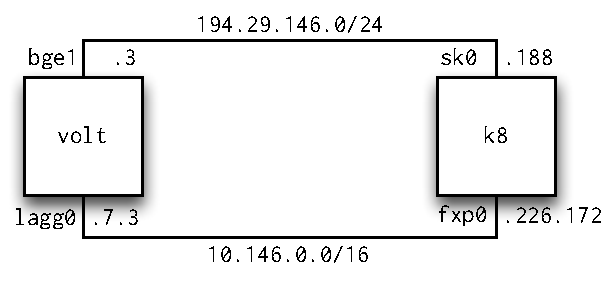
\includegraphics{figury/ethernet/schemat-po-konfiguracji.pdf}
  \caption{Schemat połączeń \eth{} po konfiguracji dodatkowego interfejsu na maszynie \kosiem.}
  \label{fig:eth:schemat-po-konfiguracji}
\end{figure}

Najpierw załadowano sterowniki do karty sieciowej firmy Intel. Nazwę modułu
znaleziono w instrukcji po wywołaniu skryptu \texttt{sterowniki -e}.

\begin{lstlisting}
k8% sudo kldload if_fxp
k8% ifconfig -a
[...]
fxp0: flags=8802<BROADCAST,SIMPLEX,MULTICAST> metric 0 mtu 1500
    options=2009<RXCSUM,VLAN_MTU,WOL_MAGIC>
    ether 00:d0:b7:0b:d2:fe
    media: Ethernet autoselect (100baseTX <full-duplex>)
    status: active
\end{lstlisting}

Po załadowaniu sterowników, zauważono powstanie nowego interfejsu o nazwie
\texttt{fxp0}. Użyliśmy programu \texttt{dhclient} by automatycznie
skonfigurować interfejs.

\begin{lstlisting}
k8% sudo dhclient fxp0
DHCPDISCOVER on fxp0 to 255.255.255.255 port 67 interval 6
DHCPDISCOVER on fxp0 to 255.255.255.255 port 67 interval 12
DHCPOFFER from 10.146.7.3
unknown dhcp option value 0xaf
DHCPREQUEST on fxp0 to 255.255.255.255 port 67
DHCPACK from 10.146.7.3
unknown dhcp option value 0xaf
bound to 10.146.226.172 -- renewal in 1800 seconds.

k8% ifconfig fxp0
fxp0: flags=8843<UP,BROADCAST,RUNNING,SIMPLEX,MULTICAST> metric 0 mtu 1500
    options=2009<RXCSUM,VLAN_MTU,WOL_MAGIC>
    ether 00:d0:b7:0b:d2:fe
    inet 10.146.226.172 netmask 255.255.0.0 broadcast 10.146.255.255
    media: Ethernet autoselect (100baseTX <full-duplex>)
    status: active

k8% netstat -r -f inet
Routing tables
Internet:
Destination        Gateway            Flags    Refs      Use  Netif Expire
default            gate               UGS         0        0    sk0
10.146.0.0         link#4             U           0        0   fxp0
10.146.226.172     link#4             UHS         0        0    lo0
localhost          link#3             UH          0        0    lo0
194.29.146.0       link#1             U           0    11770    sk0
k8.iem.pw.edu.pl   link#1             UHS         0        0    lo0
\end{lstlisting}

Widoczny jest proces nadawania adresu IP dla interfejsu. Adres został nadany
przez serwer DHCP z adresem \texttt{10.146.7.3}. Jest to adres \volt. Następnie
sprawdzono czy interfejs został skonfigurowany oraz czy tablice routingu zostały
odświeżone. Po sprawdzeniu konfiguracji przetestowano przepływ pakietów do
interfejsu. Z maszyny \volt{} wysłano 3 zapytania programem \texttt{ping}. Na
maszynie \kosiem{} programem \texttt{tcpdump} nasłuchiwano przychodzące pakiety
ICMP.

\begin{lstlisting}
# Z maszyny `volt` wysylano pakiety na adres przypisany
# maszynie `k8` przez serwer DHCP.
volt% ping -c 3 10.146.226.172
PING 10.146.226.172 (10.146.226.172): 56 data bytes
64 bytes from 10.146.226.172: icmp_seq=0 ttl=64 time=0.274 ms
64 bytes from 10.146.226.172: icmp_seq=1 ttl=64 time=0.249 ms
64 bytes from 10.146.226.172: icmp_seq=2 ttl=64 time=0.249 ms

--- 10.146.226.172 ping statistics ---
3 packets transmitted, 3 packets received, 0.0% packet loss
round-trip min/avg/max/stddev = 0.249/0.257/0.274/0.012 ms

# Na maszynie `k8` pakiety zostaly odebrane i odpowiedzi
# zostaly wyslane.
k8% sudo tcpdump -i fxp0 icmp
listening on fxp0, link-type EN10MB (Ethernet), capture size 65535 bytes
00:40:01.864733 IP 10.146.7.3 > 10.146.226.172: ICMP echo request, id 12044, seq 0, length 64
00:40:01.864766 IP 10.146.226.172 > 10.146.7.3: ICMP echo reply, id 12044, seq 0, length 64
00:40:02.866075 IP 10.146.7.3 > 10.146.226.172: ICMP echo request, id 12044, seq 1, length 64
00:40:02.866108 IP 10.146.226.172 > 10.146.7.3: ICMP echo reply, id 12044, seq 1, length 64
00:40:03.867117 IP 10.146.7.3 > 10.146.226.172: ICMP echo request, id 12044, seq 2, length 64
00:40:03.867146 IP 10.146.226.172 > 10.146.7.3: ICMP echo reply, id 12044, seq 2, length 64
^C
6 packets captured
63 packets received by filter
0 packets dropped by kernel
\end{lstlisting}

Konfiguracja przeszła testy pomyślnie. Dodatkowo nadano interfejsowi
\texttt{fxp0} drugi adres korzystając z opcji \texttt{alias} programu
\texttt{ifconfig}. By nie ryzykować zaburzenia pracy sieci jako drugi wybrano
adres z puli adresów sieci już skonfigurowanej tj. przypisano interfejsowi
\texttt{fxp0} statycznie adres \texttt{10.146.226.173/24}.

\begin{lstlisting}
k8% sudo ifconfig fxp0 alias 10.146.226.173/24
k8% ifconfig fxp0
fxp0: flags=8843<UP,BROADCAST,RUNNING,SIMPLEX,MULTICAST> metric 0 mtu 1500
    options=2009<RXCSUM,VLAN_MTU,WOL_MAGIC>
    ether 00:d0:b7:0b:d2:fe
    inet 10.146.226.172 netmask 255.255.0.0 broadcast 10.146.255.255
    inet 10.146.226.173 netmask 255.255.255.0 broadcast 10.146.226.255
    media: Ethernet autoselect (100baseTX <full-duplex>)
    status: active

k8% netstat -r
Routing tables
Internet:
Destination        Gateway            Flags    Refs      Use  Netif Expire
default            gate               UGS         0        0    sk0
10.146.0.0         link#4             U           0       11   fxp0
10.146.226.0       link#4             U           0        0   fxp0
10.146.226.172     link#4             UHS         0        0    lo0
10.146.226.173     link#4             UHS         0        0    lo0
localhost          link#3             UH          0        0    lo0
194.29.146.0       link#1             U           0    16644    sk0
k8.iem.pw.edu.pl   link#1             UHS         0        0    lo0
\end{lstlisting}

W tablicy routingu pojawiły się dwie nowe pozycje. Widać, że pakiety kierowane
do sieci \texttt{10.146.0.0/16} i \texttt{10.146.226.0/24} będą przechodziły
przez jeden interfejs.

Na koniec pracy z \eth{} usunięto konfigurację interfejsu \texttt{fxp0} i
odładowano sterowniki do karty sieciowej, z której interfejs korzystał.

\begin{lstlisting}
k8% sudo ifconfig fxp0 delete
k8% sudo kldunload if_fxp
k8% ifconfig fxp0
ifconfig: interface fxp0 does not exist
\end{lstlisting}
